\documentclass[12pt]{article}

\usepackage{sbc-template}
\usepackage{graphicx,url}
\usepackage[utf8]{inputenc}
\usepackage[brazil]{babel}

\sloppy

\title{Segmentação de texturas urbanas com um banco de\\
  filtros orientados em três escalas}

\author{Vitor Lorenzo Cumim\inst{1}}

\address{Universidade Federal do Paraná (UFPR) --
  Visão Computacional, Trabalho 1
  \email{vlc22@inf.ufpr.br}
}

\begin{document}

\maketitle

\begin{abstract}
  This work builds a 24-dimensional texture descriptor from a bank of seven
  filters --- four even-phase Gabor filters oriented at 0, 45, 90 and 135
  degrees, two odd-phase Gabor filters and one circular Laplacian of Gaussian
  --- applied over three levels of a Gaussian pyramid. Each region is
  described by the mean filter response inside a window. A hand-written
  Euclidean k-means groups 40 grayscale crops of 512x512 pixels from eight
  urban materials, reaching a purity of 0.58 against the photographed
  material, and segments the interior of each image.
\end{abstract}

\begin{resumo}
  Este trabalho monta um descritor de textura de 24 dimensões a partir de um
  banco de sete filtros --- quatro Gabor de fase par nas orientações 0, 45, 90
  e 135 graus, dois Gabor de fase ímpar e um filtro circular (Laplaciano da
  gaussiana) --- aplicados em três escalas de uma pirâmide gaussiana. Cada
  região é descrita pela média das respostas dentro de uma janela. Um k-médias
  euclidiano escrito à mão agrupa 40 recortes de 512x512 pixels em tons de
  cinza, de oito materiais urbanos, com pureza de 0,58 em relação ao material
  fotografado, e segmenta o interior de cada imagem.
\end{resumo}

\section{Introdução}

Duas regiões de uma imagem em tons de cinza podem ter exatamente o mesmo
histograma e ainda assim serem visivelmente diferentes. Uma parede de tijolos
e um trecho de asfalto podem ter o mesmo brilho médio, mas a parede tem linhas
horizontais fortes e o asfalto não tem direção nenhuma. É essa diferença ---
como a intensidade varia no espaço, em que direção e em que tamanho --- que
chamamos de textura.

A estratégia clássica para medi-la é passar a imagem por filtros sintonizados
em diferentes orientações e frequências e observar quanta energia cada um
capta \cite{jain:91,randen:99}. Este trabalho segue essa receita, com filtros
de Gabor \cite{gabor:46} e um filtro circular, para agrupar 40 imagens por
semelhança de textura e segmentar o interior de cada uma. Nenhuma etapa usa
aprendizado de máquina: os filtros são fixos e projetados analiticamente, e o
agrupamento é um k-médias euclidiano implementado diretamente. O código e as
imagens estão em \url{https://github.com/vitorcumim/textura-urbana}.

\section{Conjunto de imagens}

O conjunto é de texturas urbanas: asfalto, brita, calçada, concreto, madeira,
paralelepípedo, telha e tijolo --- oito classes, cinco imagens cada, 40
imagens no total. As fotos vieram do Wikimedia Commons, sob licenças livres,
com autor e licença registrados no repositório; cabe a ressalva de que o
enunciado pede fotos tiradas pelo próprio grupo, e estas não são. Foram
baixadas 89 candidatas e todas passaram por curadoria visual, porque a busca
textual do acervo é pouco confiável: pedir \textit{asphalt texture} devolve
cartas de ruído usadas para calibrar \textit{scanners}.

Cada foto aprovada é convertida para tons de cinza pela fórmula da ITU-R
BT.601, $Y = 0{,}299R + 0{,}587G + 0{,}114B$, e recortada em blocos de 512x512
tomados de uma grade centrada, sem sobreposição, de modo que dois recortes da
mesma foto nunca compartilhem pixels.

\section{O banco de filtros e as três escalas}

Um filtro de Gabor é uma onda cosseno (ou seno) multiplicada por uma
envoltória gaussiana, e responde forte onde a imagem tem variação periódica na
orientação e no comprimento de onda para os quais foi sintonizado. Usou-se
$\lambda = 5$ px, $\sigma = 2{,}2$ px, razão de aspecto $\gamma = 0{,}5$ e
núcleo de 15x15 px. O banco tem sete filtros: quatro Gabor de \textbf{fase
par} (cosseno) a 0, 45, 90 e 135 graus, que têm lobo central e portanto
detectam \textit{linha}, cobrindo as quatro orientações pedidas no enunciado;
dois Gabor de \textbf{fase ímpar} (seno) a 0 e 90 graus, antissimétricos, que
detectam \textit{borda} --- a distinção importa porque uma parede de tijolos e
um ripado de madeira podem ter a mesma orientação dominante e ainda assim
serem coisas diferentes; e um \textbf{filtro circular}, o Laplaciano da
gaussiana, isotrópico, que responde a granulação sem direção preferida e é
quem caracteriza asfalto e brita. Todos têm média zero, então nenhum responde
a brilho constante.

\begin{figure}[htb]
\centering
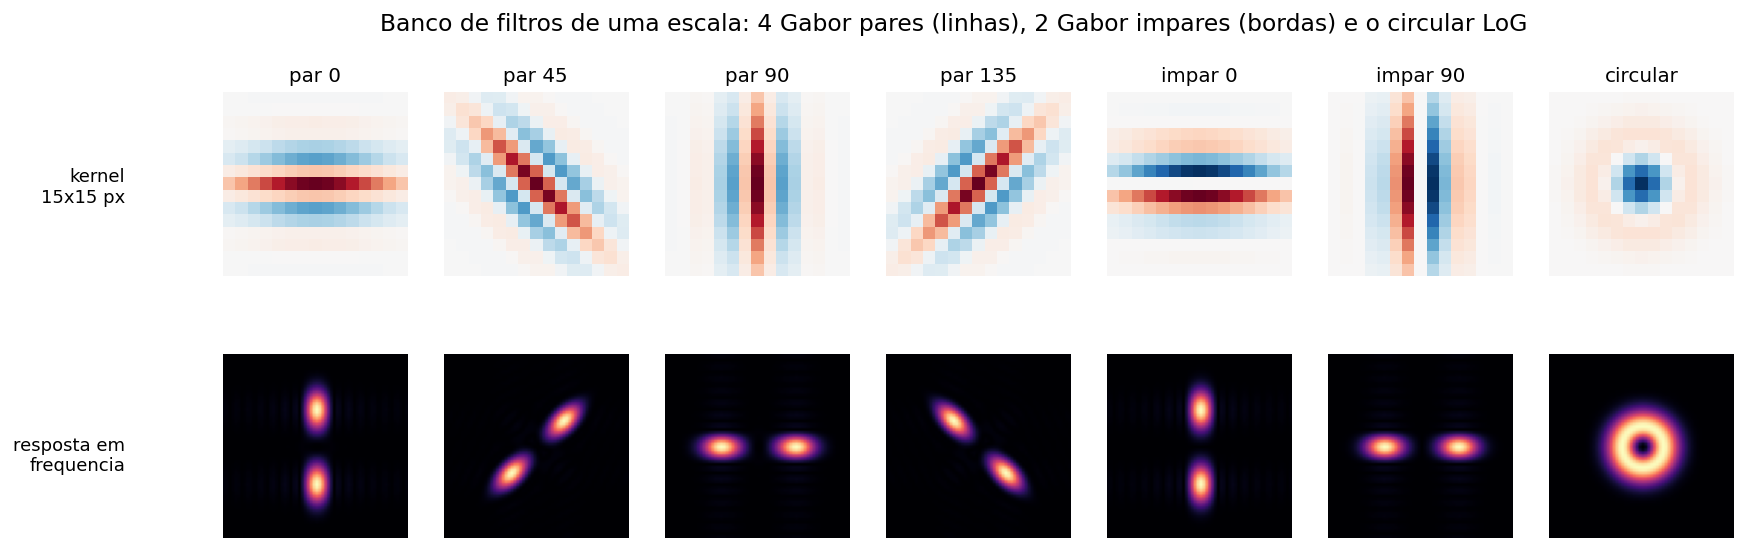
\includegraphics[width=\textwidth]{figuras/fig1_banco.png}
\caption{Os sete filtros de uma escala. Em cima o núcleo 15x15 (vermelho
  positivo, azul negativo); embaixo o módulo da resposta em frequência, onde
  cada Gabor aparece como um par de lobos na direção correspondente e o
  circular como um anel.}
\label{fig:banco}
\end{figure}

Para o multiescala, o enunciado permite construir os filtros em três tamanhos
ou construí-los uma vez e encolher a imagem. Adotou-se o segundo, mais barato.
A pirâmide gaussiana suaviza com $\sigma = 1{,}0$ e amostra um pixel a cada
dois, dando níveis de 512x512, 256x256 e 128x128; como o filtro continua
15x15, no nível 2 ele enxerga uma vizinhança quatro vezes maior da imagem
original. Sete filtros em três escalas produzem 21 mapas de resposta. De cada
mapa toma-se o valor absoluto, porque uma barra clara sobre fundo escuro e uma
barra escura sobre fundo claro são a mesma textura, e sem retificar a média da
janela daria aproximadamente zero para as duas.

\section{O descritor de 24 dimensões}

O descritor de uma região é a média de cada mapa de resposta dentro da janela,
o que dá 21 números. Usá-los crus não funciona bem: eles carregam o contraste
da foto, e a distância euclidiana passa a medir \textit{quanto contraste a
imagem tem} em vez de \textit{que textura ela é} --- a mesma parede ao sol e na
sombra vira dois grupos.

A correção é separar as duas coisas. Cada escala passa a ser descrita por oito
números: as sete frações $r_i / (r_1 + \cdots + r_7)$, que dizem como a energia
se reparte entre as orientações e o filtro circular --- a \textit{forma} da
assinatura, invariante a contraste --- e o valor $\log(1 + r_1 + \cdots + r_7)$,
a energia total daquela escala, isto é, o \textit{tamanho}. Três escalas por
oito números dão as 24 dimensões. A Tabela~\ref{tab:descritor} mostra o ganho
medido, mudando apenas a forma do descritor.

\begin{table}[htb]
\centering
\caption{Efeito da forma do descritor sobre a pureza do agrupamento.}
\label{tab:descritor}
\begin{tabular}{lcc}
\hline
\textbf{Descritor} & \textbf{Dimensões} & \textbf{Pureza (k=8)} \\
\hline
médias cruas dos filtros e passa-baixa  & 24 & 0,40 \\
médias cruas, sem a passa-baixa         & 21 & 0,45 \\
logaritmo das médias cruas              & 24 & 0,50 \\
perfil normalizado e energia por escala & 24 & \textbf{0,58} \\
\hline
\end{tabular}
\end{table}

O mesmo cálculo serve em duas granularidades. Com a imagem inteira como
janela, sai um vetor por imagem, usado para agrupar o conjunto. Com janelas de
64x64 px andando de 32 em 32 px, saem 225 vetores por imagem, usados para
segmentar por dentro; a janela é maior que o passo de propósito, porque com
janelas justas de 32x32 o mapa de rótulos fica pipocado.

\section{Agrupamento e resultados}

O agrupamento é um k-médias euclidiano implementado à mão, com inicialização
k-means++ \cite{arthur:07}, semente fixa e dez reinicializações, ficando com a
de menor inércia. Antes, cada dimensão passa por z-score: as frações vivem
entre 0 e 1 e a energia logarítmica vale alguns inteiros, então sem normalizar
a distância seria dominada pelas dimensões de energia.

Nem a inércia nem a silhueta indicam um k natural --- as texturas urbanas
formam um contínuo, não oito nuvens separadas. Adotou-se k = 8, o número de
materiais fotografados, que dá pureza 0,575 e silhueta 0,220. A pureza é a
fração de imagens que está no rótulo majoritário do seu grupo, e é preciso
lembrar que ela pune o método quando ele está certo mas discorda da etiqueta:
um concreto muito granulado realmente se parece mais com brita do que com um
concreto liso.

\begin{table}[htb]
\centering
\caption{Composição dos oito grupos encontrados.}
\label{tab:grupos}
\begin{tabular}{clp{7.2cm}}
\hline
\textbf{Grupo} & \textbf{n} & \textbf{O que reuniu} \\
\hline
G0 & 7 & superfícies granuladas de contraste médio \\
G1 & 1 & tapume claro de ripas verticais \\
G2 & 3 & veio de madeira horizontal \\
G3 & 2 & telhas em fiadas diagonais \\
G4 & 9 & alvenaria: blocos com juntas horizontais fortes \\
G5 & 5 & superfícies lisas de granulação fina \\
G6 & 9 & granulado grosso e sem direção \\
G7 & 4 & placas grandes e lisas separadas por juntas largas \\
\hline
\end{tabular}
\end{table}

A pureza de 0,575 esconde um comportamento que a Figura~\ref{fig:grupos} torna
evidente: os grupos são coerentes como textura, ainda quando não coincidem com
o material. G6 junta as cinco britas com concretos granulados e paralelepípedos
rugosos --- todos são granulação grossa isotrópica, e o filtro circular os vê
como a mesma coisa. G4 junta tijolo, calçada em blocos e telha em fiadas, que
são todos retângulos separados por juntas horizontais. Os erros que restam são
de dois tipos: a classe que se parte, como as telhas, espalhadas por três
grupos porque telha de frente, em diagonal e empilhada são texturas diferentes
com o mesmo nome; e os grupos de um elemento só, de imagens atípicas demais
para se juntar a qualquer outra.

\begin{figure}[p]
\centering
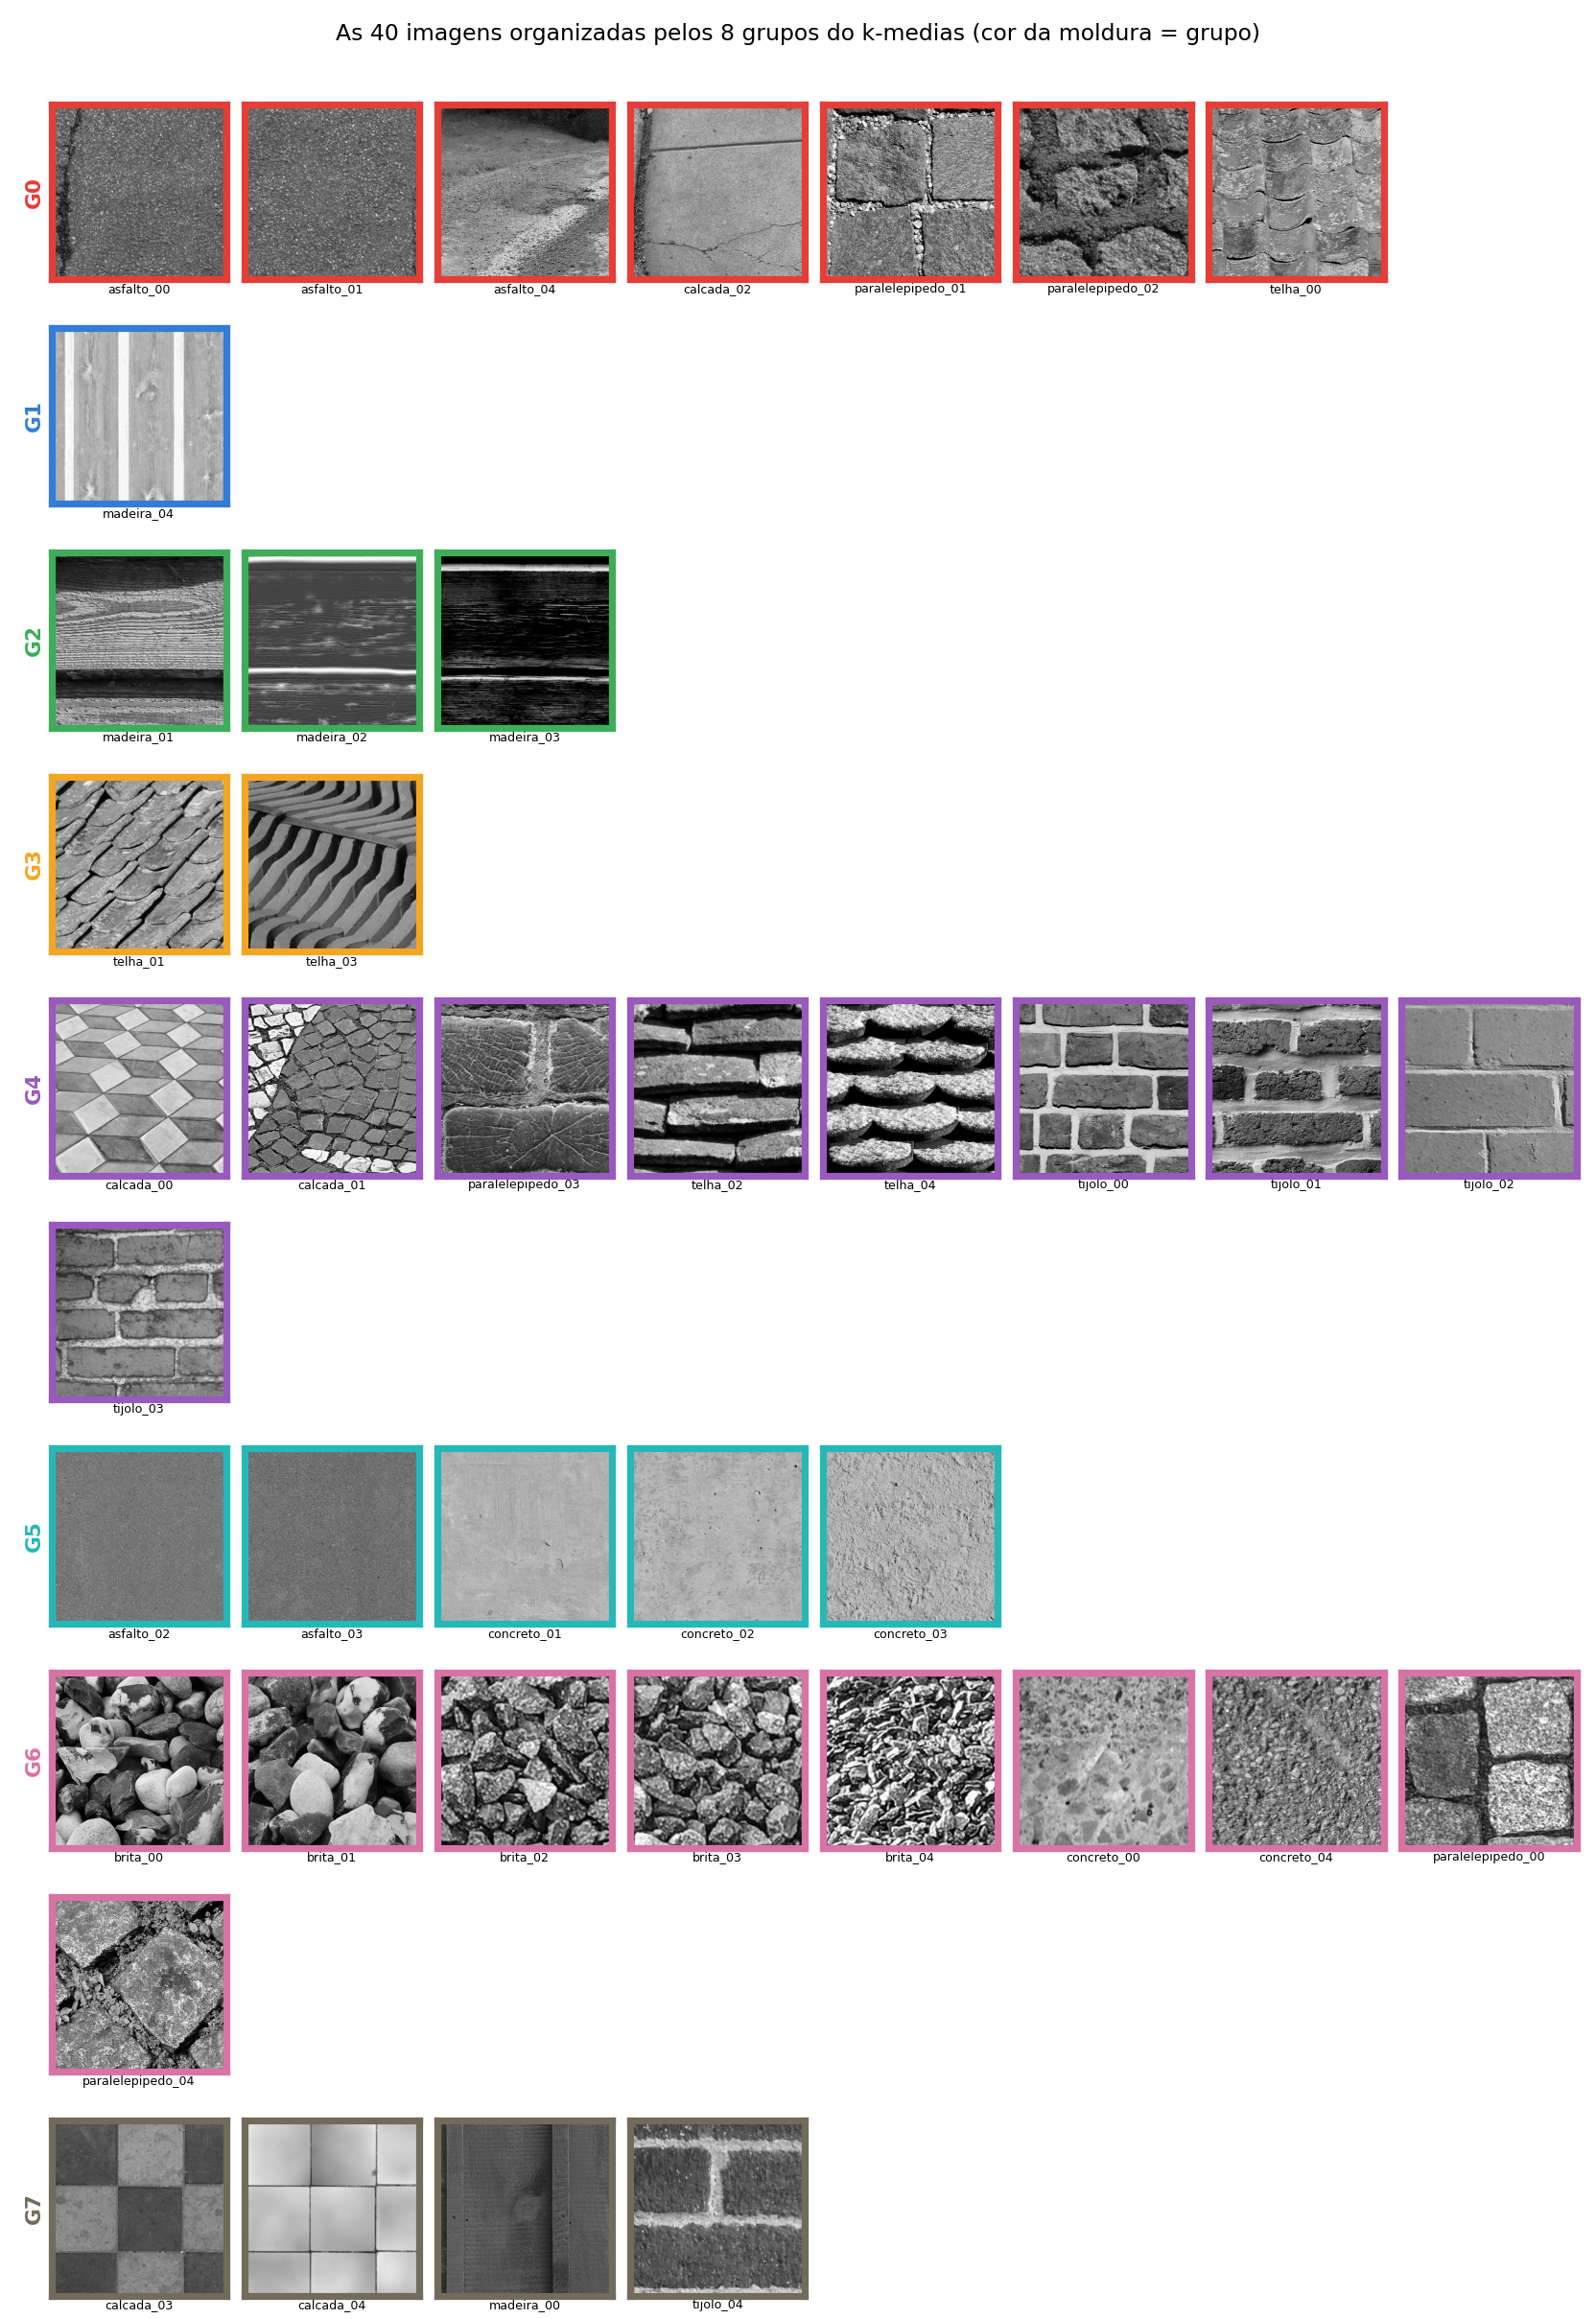
\includegraphics[width=\textwidth]{figuras/fig4_grupos.png}
\caption{As 40 imagens organizadas pelos oito grupos do k-médias. A cor da
  moldura indica o grupo.}
\label{fig:grupos}
\end{figure}

Rodando o mesmo k-médias sobre as 9.000 janelas de 64x64 de todas as imagens,
com k = 6, cada janela recebe o rótulo do grupo mais próximo, o que produz um
mapa de segmentação por textura (Figura~\ref{fig:segmentacao}). Este é o
resultado mais fácil de auditar a olho: as regiões que o método separa --- as
frestas entre ripas de madeira, o rejunte entre as pedras, a junta entre
placas de concreto --- são as que uma pessoa apontaria. O mapa é grosseiro por
construção, com limites em degraus de 32 px.

\begin{figure}[htb]
\centering
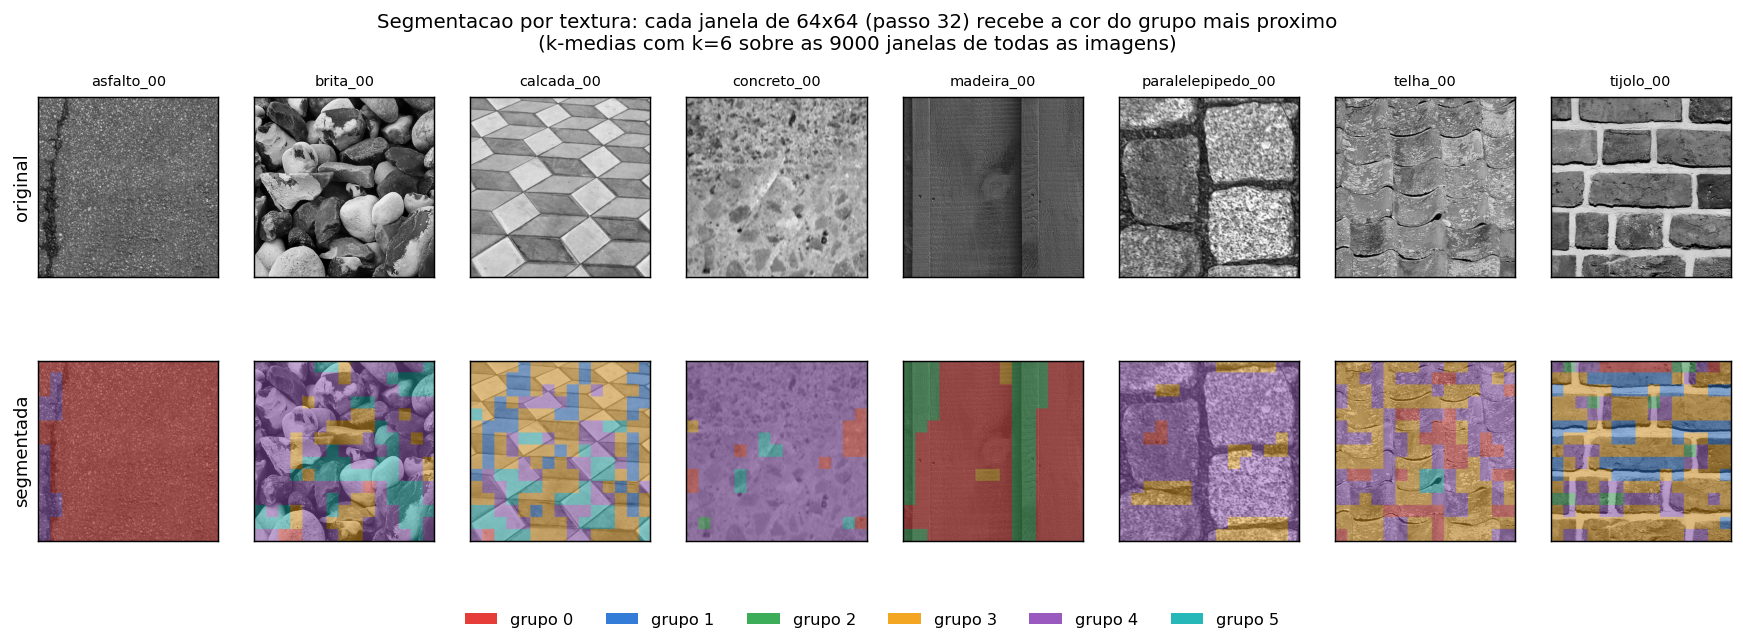
\includegraphics[width=0.95\textwidth]{figuras/fig7_segmentacao.png}
\caption{Segmentação por textura: acima as imagens originais, abaixo o mapa de
  grupos sobreposto. Uma imagem de textura uniforme fica quase toda de uma cor
  só; onde há mais de um material, o limite aparece.}
\label{fig:segmentacao}
\end{figure}

Para verificar quanto o resultado depende do banco escolhido, todo o
\textit{pipeline} foi repetido com derivadas de gaussiana
\cite{freeman:91} --- 2ª derivada no lugar do Gabor par, 1ª derivada no lugar
do ímpar, mesmo filtro circular --- mantendo idênticos o conjunto, a pirâmide,
o descritor e o agrupamento. A troca quase não muda nada: mesma pureza, índice
de Rand \cite{rand:71} de 0,98 entre os dois agrupamentos e uma única imagem
das 40 trocando de grupo. O descritor descarta a diferença, porque a média do módulo numa janela
de 64x64, depois normalizada pela energia, dá quase o mesmo número vindo de
filtros diferentes.

\section{Limitações e conclusão}

O método não tem invariância a rotação --- girar a foto 45 graus muda o
descritor por completo, consequência de usar orientações fixas --- nem a
escala de aquisição, já que as três escalas cobrem uma faixa de apenas 4x. O k
foi escolhido à mão, por corresponder ao número de materiais, que é informação
externa ao método. E o conjunto é pequeno: 40 imagens vindas de 36 fotos.

Ainda assim, um banco de sete filtros orientados aplicado em três escalas e
resumido pela média das respostas em cada janela é suficiente para agrupar
texturas urbanas de maneira visualmente coerente e para segmentar o interior
das imagens sem nenhum aprendizado. O passo que mais afetou o resultado não
foi a escolha dos filtros, e sim a forma do descritor: separar a repartição da
energia entre os filtros da quantidade total de energia levou a pureza de 0,40
para 0,58. Trocar o banco inteiro, em contraste, deixou o resultado
essencialmente intacto.

\bibliographystyle{sbc}
\bibliography{artigo}

\end{document}
